\documentclass[11pt]{article}
% Shared preamble for the notes in this repository. pdfLaTeX, TeX Live 2024 or later.
\usepackage[a4paper,margin=2.6cm]{geometry}
\usepackage[T1]{fontenc}
\usepackage{lmodern}
\usepackage{microtype}
\usepackage{amsmath,amssymb,amsthm}
\usepackage{graphicx}
\usepackage{booktabs}
\usepackage{enumitem}
\usepackage[dvipsnames]{xcolor}
\usepackage[hidelinks]{hyperref}
\hypersetup{colorlinks=true,linkcolor=MidnightBlue,citecolor=MidnightBlue,urlcolor=MidnightBlue}
\graphicspath{{../../figures/}}
\setlist{itemsep=2pt,topsep=4pt}

\newtheorem{theorem}{Theorem}
\newtheorem{proposition}[theorem]{Proposition}
\newtheorem{corollary}[theorem]{Corollary}
\newtheorem{conjecture}[theorem]{Conjecture}
\theoremstyle{definition}
\newtheorem{definition}[theorem]{Definition}
% Reusable derivations, numbered note.k; each note sets \notenumber. Indexed in DERIVATIONS.md.
\newcommand{\notenumber}{0}
\newtheorem{derivation}{Derivation}
\renewcommand{\thederivation}{\notenumber.\arabic{derivation}}
\newtheorem{question}{Question}
\theoremstyle{remark}
\newtheorem{remark}[theorem]{Remark}

\newcommand{\Z}{\mathbb{Z}}
\newcommand{\Q}{\mathbb{Q}}
\newcommand{\R}{\mathbb{R}}
\newcommand{\C}{\mathbb{C}}
\newcommand{\HH}{\mathbb{H}}
\newcommand{\SL}{\mathrm{SL}}
\newcommand{\Gal}{\mathrm{Gal}}
\newcommand{\Hom}{\mathrm{Hom}}
\newcommand{\repo}{\href{https://github.com/rmorleysmith/l-functions-and-physics}{\texttt{l-functions-and-physics}}}
\newcommand{\formal}{\href{https://github.com/rmorleysmith/morley-smith-formal}{\texttt{morley-smith-formal}}}
\newcommand{\script}[1]{\href{https://github.com/rmorleysmith/l-functions-and-physics/blob/main/scripts/#1}{\texttt{scripts/#1}}}
% A path inside the Lean repository; it may break after a slash.
\newcommand{\leanpath}[1]{\nolinkurl{#1}}

% Grades used in every status table.
\newcommand{\gradeLean}{\textsc{lean}}      % proved in Lean 4 with Mathlib
\newcommand{\gradeClassical}{\textsc{classical}}  % a published theorem, cited
\newcommand{\gradeComputed}{\textsc{computed}}    % checked numerically by a script in this repository
\newcommand{\gradeConvention}{\textsc{convention}}  % a choice of units or names
\newcommand{\gradeOpen}{\textsc{open}}      % a question, conjecture or working hypothesis
% The legend printed under every status table.
\newcommand{\gradelegend}{\par\nopagebreak\smallskip\noindent\begin{minipage}{\textwidth}\small
\gradeLean: proved in Lean 4 with Mathlib.
\gradeClassical: a published theorem.
\gradeComputed: checked numerically by a script in the repository \repo.
\gradeConvention: a choice of units or names.
\gradeOpen: a question, conjecture or working hypothesis.
\end{minipage}\par\medskip}
% A plain-language physical reading, placed after each derivation.
\newcommand{\physical}{\paragraph{In physical terms.}}

\renewcommand{\notenumber}{10}

\title{Spheres: echoes, multipoles and rotations}
\author{Richard Morley-Smith}
\date{Note 10 \quad November 2026}

\begin{document}
\maketitle

\begin{abstract}
\noindent
A lattice of unit impulses in space can be taken apart in two ways: by distance, into shells, and by direction, into spherical harmonics.
We follow both.
A flash at every site of a cubic lattice returns to a site as a train of echoes at the times $\sqrt N$; for squarefree $N$ the strength of the echo is a Dirichlet $L$-value divided by $\zeta(2)$, the echoes at $N = 7, 15, 23, 28,\dots$ are missing, and the same integers weight the echoes and the normal modes.
The shape of a shell is carried by its multipole moments, and these are the coefficients of modular forms of weight $l+d/2$.
The first of them, the hexadecapole of the $N$-th shell of $\Z^d$, is the coefficient of an eta product for $d = 2,3,4$, and the crystal field of a cubic lattice of charges is the field of the nearest neighbours times $0.888\,064\,766\ldots$, a value of its Dirichlet series.
In space the square of the hexadecapole is the central value of an $L$-function, so the size of a shell is an $L$-value at the edge of the critical strip and its shape an $L$-value at the centre.
In four dimensions shells are as round as chance allows, their anisotropy about one over the square root of the number of points: this is Deligne's theorem. In space the same rate is a Lindel\"of hypothesis, and it holds in the median of the computation.
On the three-sphere, whose harmonics are the shells of the hydrogen atom, the spin states fixed by the 24 Hurwitz units are Klein's octahedron and cube, and they are counted by the newforms of level~2.
Finally, the six rotations given by the quaternions $1\pm2i$, $1\pm2j$, $1\pm2k$ mix the sphere at the rate $2\sqrt5$ of the Ramanujan bound; they are gates for a quantum bit.
\end{abstract}

\section{The packets of a sphere}

\begin{derivation}[harmonic packets]\label{d:packets}
Let $\mathcal H_l(\R^d)$ be the homogeneous polynomials $P$ of degree $l$ in $d$ variables with $\Delta P = 0$.
Every polynomial, restricted to the unit sphere, is a sum of harmonic ones in exactly one way, and
\[
  \dim\mathcal H_l(\R^d) = \binom{l+d-1}{d-1}-\binom{l+d-3}{d-1} =
  \begin{cases} 2 & d=2,\ l\ge1,\\ 2l+1 & d=3,\\ (l+1)^2 & d=4.\end{cases}
\]
On the sphere, $\mathcal H_l$ is the eigenspace of the Laplacian with eigenvalue $-l(l+d-2)$, and harmonics of different degrees are orthogonal \cite{SteinWeiss}.
\end{derivation}

\physical
The degree $l$ is the angular momentum, and a function on a sphere is a sum of orthogonal packets, one for each $l$: monopole, dipole, quadrupole, octupole, hexadecapole for $l = 0,\dots,4$; the $s$, $p$, $d$, $f$ orbitals of an atom for $l = 0,\dots,3$.
In four dimensions the count $(l+1)^2 = n^2$, with $n = l+1$, is the degeneracy of the level $n$ of hydrogen: Fock showed that the bound states of hydrogen, written in momentum space, are the harmonics on the three-sphere \cite{Fock, BanderItzykson}.
The three-sphere is the group of unit quaternions, which acts on itself from the left and from the right, and $\mathcal H_l(\R^4)$ is the product $V_l\otimes V_l$ of two spins $l/2$.

\section{Echoes of a cubic lattice}

Write $r_d(N)$ for the number of $x\in\Z^d$ with $|x|^2 = N$.
The numbers $r_3(N)$, which begin $6$, $12$, $8$, $6$, $24$, $24$, $0$, $12$, $30$, are the numbers of $N$-th neighbours of an atom in a simple cubic crystal.

\begin{derivation}[echoes]\label{d:echoes}
Let $u$ solve the wave equation $u_{tt} = c^2\Delta u$ in $\R^3$ with $u = 0$ and $u_t = \sum_{n\in\Z^3}\delta(x-an)$ at $t=0$: a unit flash at every site of a cubic lattice of spacing $a$.
A single flash has the response $\delta(|x|-ct)/(4\pi c|x|)$ (Kirchhoff's formula \cite{Evans}), so at a lattice site and for $t>0$
\[
  u(0,t) = \frac{1}{4\pi c^2a}\sum_{N\ge1}\frac{r_3(N)}{\sqrt N}\,\delta\Big(t-\frac{a\sqrt N}{c}\Big).
\]
In units with $a = c = 1$, the same signal is a sum over the normal modes of the torus $\R^3/\Z^3$:
\[
  \sum_{N\ge1}\frac{r_3(N)}{4\pi\sqrt N}\,\delta(t-\sqrt N) \;=\; t+\sum_{N\ge1}r_3(N)\,\frac{\sin(2\pi\sqrt N\,t)}{2\pi\sqrt N}\qquad(t>0),
\]
which is Poisson summation for radial functions in three dimensions.
For squarefree $N\not\equiv7\pmod 8$, with $D$ the discriminant of $\Q(\sqrt{-N})$,
\[
  \frac{r_3(N)}{4\pi\sqrt N} = \frac{L(1,\chi_D)}{\zeta(2)},
\]
and $r_3(N) = 0$ exactly when $N = 4^a(8b+7)$ (Gauss; Legendre \cite{Grosswald}).
\end{derivation}

\physical
An observer at a lattice site hears the $N$-th shell of neighbours at the time $a\sqrt N/c$.
For squarefree $N$ the loudness of that echo is a Dirichlet $L$-value at $s=1$ divided by $\zeta(2)$, and the echoes numbered $7, 15, 23, 28, 31,\dots$ are missing (Figure~\ref{fig:echoes}).
The left side of the second formula lists echoes and the right side lists tones.
In the trace formula of note~09 the two lists were the primes and the zeros; for the cubic torus they are one list, the integers $r_3(N)$.
The script \script{spheres.py} checks the identity, smoothed by a Gaussian, to $10^{-13}$, and the $L$-value form for the 151 squarefree $N\le300$.
In the plane the response to a flash is $(2\pi c)^{-1}(c^2t^2-|x|^2)^{-1/2}$ inside the light cone, a front followed by a tail.
Sharp echoes need an odd number of dimensions (Huygens' principle), and three is the first.

\begin{figure}[ht]
  \centering
  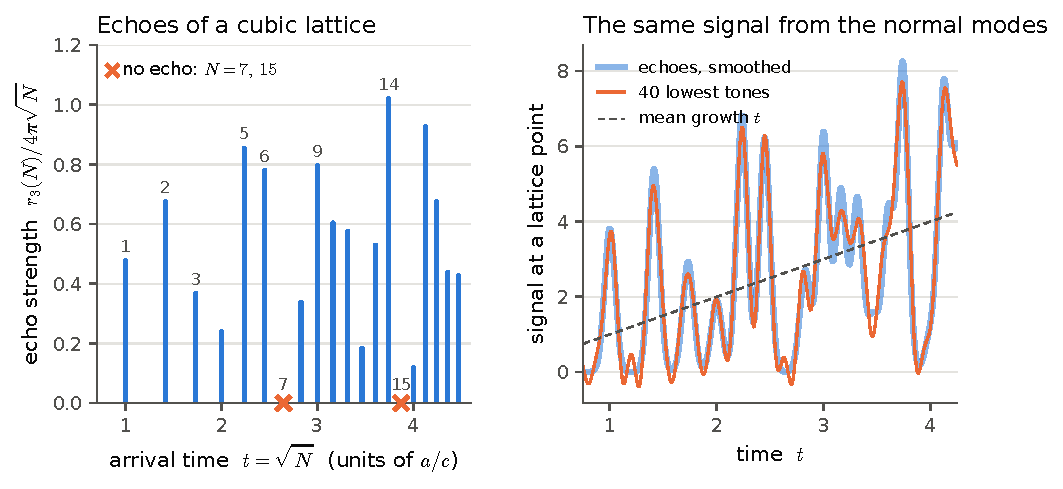
\includegraphics[width=0.94\textwidth]{spheres-echoes}
  \caption{Left: the echoes of a cubic lattice of flashes, heard at a lattice site; the numbers are $N$. Right: the echo train smoothed by a Gaussian of width $0.05$, and the sum of the mean growth $t$ and the 40 lowest normal modes. With all modes the two agree to $10^{-13}$.}
  \label{fig:echoes}
\end{figure}

\section{The shape of a shell}

\begin{derivation}[the multipoles of a shell are coefficients of modular forms]\label{d:multipoles}
For $P\in\mathcal H_l(\R^d)$ the series $\theta_P(z) = \sum_{x\in\Z^d}P(x)\,q^{|x|^2}$, $q = e^{2\pi iz}$, is a modular form of weight $l+d/2$ and level 4, and a cusp form when $l\ge1$ \cite{Schoeneberg, Shimura}.
Let $K_4(x) = \sum_i x_i^4-\frac{3}{d+2}|x|^4$, the harmonic of degree 4 with the symmetry of the cube, and $\theta(z) = \sum_{n\in\Z}q^{n^2}$.
Then
\begin{align*}
  \sum_{x\in\Z^d}K_4(x)\,q^{|x|^2} &= \frac{2d(d-1)}{d+2}\,\theta(z)^d\,\psi(z),\\
  \psi(z) &= \frac{\eta(z)^8\eta(4z)^8}{\eta(2z)^8} = \sum_{n\ge1}(-1)^{n-1}\sigma_3^{\mathrm{odd}}(n)\,q^n = q-8q^2+28q^3-64q^4+\cdots,
\end{align*}
where $\sigma_3^{\mathrm{odd}}(n)$ is the sum of $\delta^3$ over the divisors $\delta$ of $n$ with $n/\delta$ odd.
Indeed, with $\mathcal D = q\,d/dq$ the left side is $d\,\theta^{d-1}\mathcal D^2\theta-\frac{3}{d+2}\mathcal D^2(\theta^d) = \frac{d(d-1)}{d+2}\,\theta^{d-2}\big(\theta\,\mathcal D^2\theta-3(\mathcal D\theta)^2\big)$, and $\theta\,\mathcal D^2\theta-3(\mathcal D\theta)^2 = 2\theta^2\psi$ is an identity between two modular forms of weight 5, the left one a Rankin--Cohen bracket \cite{Zagier}, which finitely many coefficients decide.
\end{derivation}

\begin{center}
\small
\begin{tabular}{@{}clc@{}}
\toprule
$d$ & $\sum_{x\in\Z^d}K_4(x)\,q^{|x|^2}$ & weight\\
\midrule
2 & $\eta(z)^4\eta(2z)^2\eta(4z)^4 = q-4q^2+16q^4-14q^5-64q^8+81q^9+\cdots$ & $5$\\
3 & $\tfrac{12}{5}\,\eta(z)^2\eta(2z)^7\eta(4z)^2 = \tfrac{12}{5}\,(q-2q^2-8q^3+16q^4+20q^5-36q^6+0\,q^7-\cdots)$ & $\tfrac{11}{2}$\\
4 & $4\,\eta(2z)^{12} = 4\,(q-12q^3+54q^5-88q^7-99q^9+\cdots)$ & $6$\\
\bottomrule
\end{tabular}
\end{center}

\physical
The $l$-th multipole moment of the $N$-th shell is the $N$-th coefficient of a modular form of weight $l+d/2$.
The monopole is the size $r_d(N)$ of the shell.
The symmetry of the cube removes the dipole, the quadrupole and the octupole, so the first coefficient of shape is the hexadecapole.
Write $g = \eta(z)^2\eta(2z)^7\eta(4z)^2 = \sum a(N)q^N$ for the form of the cubic lattice in space.
Then $a(N)$ is positive when the points of the shell lean towards the axes and negative when they lean towards the diagonals: $a(4) = 16$ for the six points $(\pm2,0,0)$ and $a(3) = -8$ for the eight corners $(\pm1,\pm1,\pm1)$.
The formula reads $a(N) = \sum_{m\ge1}\psi(m)\,r_3(N-m)$: the shape of a shell is computed from the sizes of the smaller shells.
The script checks the three identities to $q^{400}$, $q^{400}$ and $q^{150}$.

\paragraph{Crystal fields.}
Six charges $q$ at distance $a$ along the axes produce near the origin the potential
$\frac{6q}{a}+\frac{35q}{4a^5}\big(x^4+y^4+z^4-\tfrac35r^4\big)+O(r^6)$.
The second term is the octahedral crystal field, which splits the $d$-levels of an ion in a crystal \cite{Bethe}.
The $N$-th shell of a cubic lattice adds the same term multiplied by $a(N)N^{-9/2}$.
For a simple cubic lattice of equal point charges the crystal field is therefore that of the nearest neighbours times
\[
  L(g,\tfrac92) = \sum_{N\ge1}\frac{a(N)}{N^{9/2}} = 0.888\,064\,766\,485\,554\ldots,
\]
and for charges of alternating sign (rock salt) times $\sum(-1)^{N-1}a(N)N^{-9/2} = 1.022\,452\,1\ldots$
The first value is computed by Ewald's method \cite{Ewald}, the splitting of a lattice sum by the theta transformation.
Here it is the functional equation $\Lambda(\tfrac{11}{2}-s) = \Lambda(s)$ of $\Lambda(s) = \pi^{-s}\Gamma(s)L(g,s)$, which pairs the value at $\tfrac92$ with the value at $1$.

\section{Size and shape as $L$-values}

\begin{derivation}[the square of a multipole is a central value]\label{d:central}
Let $F = \eta(z)^8\eta(2z)^8\,\big(2E_2(2z)-E_2(z)\big) = q+16q^2-156q^3+256q^4+870q^5-\cdots$, the newform of weight 10 and level 2.
It is the Shimura lift of $g$: its coefficients satisfy $a_F(p) = a(p^2)+\chi_{-4}(p)\,p^4$ for odd primes $p$ \cite{Shimura}.
For squarefree $N\not\equiv7\pmod8$, with $D$ the discriminant of $\Q(\sqrt{-N})$,
\[
  \frac{a(N)^2}{N^{9/2}} = \frac{L(5,F\otimes\chi_D)}{L(5,F\otimes\chi_{-4})},
\]
a ratio of central values of the twisted $L$-functions $L(s,F\otimes\chi_D) = \sum a_F(n)\chi_D(n)n^{-s}$.
By Waldspurger's theorem \cite{Waldspurger} the two sides are proportional within each class of $N$ in $\Q_2^\times$ modulo squares ($N$ modulo 8 for odd $N$, modulo 16 for even $N$).
That the constant is the same in the seven classes that occur is computed, for the 201 values $N\le400$.
For squarefree $N\equiv7\pmod8$ the functional equation of $L(s,F\otimes\chi_{-N})$ has root number $-1$, and the central value is zero.
\end{derivation}

\physical
The energy in the hexadecapole of the $N$-th shell, relative to the first shell, is the central value of an $L$-function.
With Derivation~\ref{d:echoes}, the size of a shell is an $L$-value at $s=1$, the edge of the critical strip, and the square of its shape is an $L$-value at the centre.
The empty shells are those on which the central value vanishes by symmetry.
The script checks the lift for $3\le p\le47$ and the formula for the 16 squarefree $N\le30$, to $10^{-14}$ (\script{shape\_law.py} extends this to the 201 values $N\le400$, to $10^{-11}$); the constant is $1/L(5,F\otimes\chi_{-4}) = 0.377\,316\,969$.

\begin{derivation}[how round is a shell]\label{d:round}
Let $\mu_d(N) = r_d(N)^{-1}\sum_{|x|^2=N}K_4(x/|x|)$, the mean of the cubic harmonic over the $N$-th shell of $\Z^d$.
It is zero for a shell spread evenly, and of order $1/\sqrt{\text{number of points}}$ for independent random points.
\begin{itemize}
\item $d=2$. For a prime $p = a^2+b^2$ with $a>b>0$ and $\theta_p = \arctan(b/a)$, $\mu_2(p) = \tfrac14\cos4\theta_p$. The angles $\theta_p$ are equidistributed in $(0,\pi/4)$ \cite{Hecke}.
\item $d=3$. For squarefree $N\not\equiv7\pmod8$, by Derivations~\ref{d:echoes} and~\ref{d:central} (the second computed across classes),
\[
  \mu_3(N)^2 = \frac{\pi^2}{100}\,\frac{L(5,F\otimes\chi_D)}{L(5,F\otimes\chi_{-4})\,L(1,\chi_D)^2\,\sqrt N},
\]
and $\mu_3(N)\to0$ \cite{Iwaniec87, Duke}.
\item $d=4$. For an odd prime $p$, $\mu_4(p) = a_6(p)/\big(2(p+1)p^2\big)$ with $\eta(2z)^{12} = \sum a_6(n)q^n$, and Deligne's bound $|a_6(p)|\le2p^{5/2}$ gives $|\mu_4(p)|\le\sqrt p/(p+1)$ \cite{Deligne}.
\end{itemize}
\end{derivation}

\physical
In the computations the anisotropy of a shell is about one over the square root of its number of points, the size it would have for points thrown at random (Figure~\ref{fig:round}); in four dimensions this is a theorem, and in space a conjecture.
In the plane a shell of prime radius has eight points and stays anisotropic, and the pattern turns with the prime: the angles of the 39\,175 primes $p\equiv1\pmod4$ below $10^6$ are uniform to a Kolmogorov--Smirnov distance of $0.0018$.
In space $|\mu_3|\sqrt{r_3}$ has median $0.37$ for $N\le20\,000$.
Iwaniec's bound \cite{Iwaniec87} gives the rate $N^{-1/28+\varepsilon}$; the rate $N^{-1/4+\varepsilon}$ of random points is, by the formula above, the Lindel\"of hypothesis for the central values $L(5,F\otimes\chi_D)$.
In four dimensions the random rate is a theorem: $|a_6(p)|\le2p^{5/2}$ holds for the 2261 odd primes below $20\,000$ with largest ratio $0.9983$, and $a_6(p)/2p^{5/2}$ follows the semicircle law \cite{SatoTate}.
The Ramanujan--Petersson bound on the coefficients of a cusp form of integral weight is the statement that lattice shells in four dimensions are as round as chance allows.

\begin{figure}[ht]
  \centering
  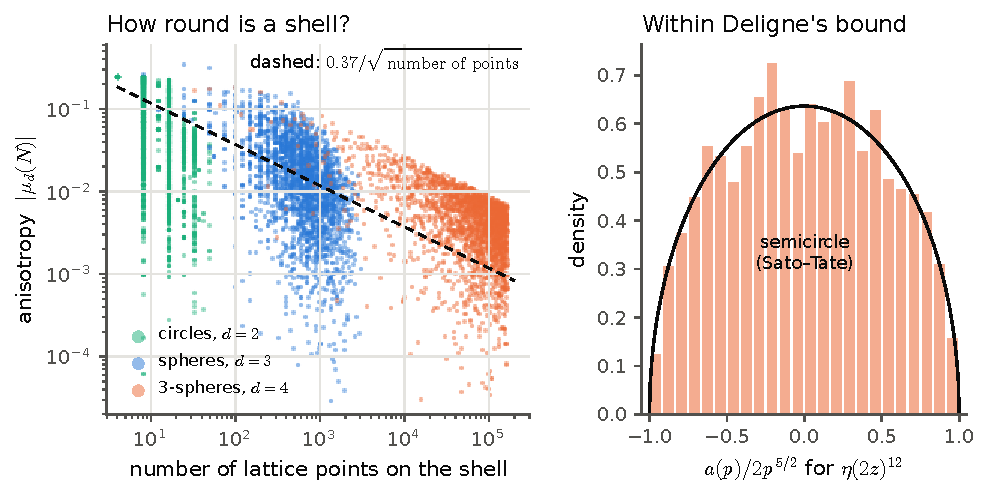
\includegraphics[width=0.94\textwidth]{spheres-roundness}
  \caption{Left: the anisotropy $|\mu_d(N)|$ of the shells of $\Z^d$ against their number of points, for circles ($N\le20\,000$), spheres (2500 shells with $200<N\le20\,000$) and three-spheres (odd primes below $20\,000$). Right: the coefficients of $\eta(2z)^{12}$ at the primes, within Deligne's bound.}
  \label{fig:round}
\end{figure}

\section{Hydrogen's shells and the Hurwitz units}

The Hurwitz quaternions are the $a+bi+cj+dk$ with $a,b,c,d$ all integers or all halves of odd integers.
There are $24\sum_{\delta\mid n,\ \delta\ \mathrm{odd}}\delta$ of norm $n$, and the 24 of norm 1 form a group: the units.
The units are the group $\SL(2,\mathbb F_3)$, the modular group reduced modulo 3, under $S\mapsto i$, $T\mapsto\frac12(-1-i+j+k)$.
Its largest abelian quotient is $\Z/3$, generated by $T$, so the characters of order 3 among the twelve of note~01 factor through the Hurwitz units.
As vectors, the units are the roots of a root system of type $D_4$, the vertices of the 24-cell.

Let $V_l$ be the binary forms of degree $l$, the states of a spin $l/2$.
A state is a constellation of $l$ points on the sphere, the roots of the form \cite{Majorana}, and the unit quaternions, as $\mathrm{SU}(2)$, rotate it.

\begin{derivation}[spin states fixed by the Hurwitz units are newforms of level 2]\label{d:hurwitz}
Let a quaternion $x = a+bi+cj+dk$ act on $V_l$ through its matrix $\left(\begin{smallmatrix}a+bi&c+di\\-c+di&a-bi\end{smallmatrix}\right)$, and write $N(x)$ for its norm.
\begin{enumerate}[label=(\roman*)]
\item The forms fixed by the 24 units are the polynomials in Klein's forms
$\Phi = u^5v-uv^5$, $\Psi = u^8+14u^4v^4+v^8$ and $X = u^{12}-33u^8v^4-33u^4v^8+v^{12}$, with $X^2 = \Psi^3-108\,\Phi^4$.
The number $m_l$ of independent ones of degree $l$ has generating function $\sum_l m_lt^l = (1+t^{12})/\big((1-t^6)(1-t^8)\big)$ \cite{Klein}.
\item For $l\ge1$, $m_l$ is the number of newforms of weight $l+2$ and level 2 \cite{Eichler, JacquetLanglands}.
\item For a fixed form $v$ of degree $l\ge1$, the series $\sum_x\langle v,x\cdot v\rangle\,q^{N(x)}$ over the Hurwitz quaternions $x$ is a cusp form of weight $l+2$ and level 2.
For $v = \Phi,\Psi,X,\Phi^2$ it is a multiple of the newform in the table below.
\item In each of these four cases the twist $(1+i)/\sqrt2$ multiplies $v$ by $\varepsilon = \pm1$, and the newform has $a(2) = \varepsilon\,2^{l/2}$ and root number $(-1)^{l/2}\varepsilon$.
\end{enumerate}
\end{derivation}

\begin{center}
\small
\begin{tabular}{@{}llclcc@{}}
\toprule
state & stars & weight & newform of level 2 & $\varepsilon$ & root no.\\
\midrule
$\Phi$, spin 3 & octahedron & 8 & $\eta(z)^8\eta(2z)^8 = q-8q^2+12q^3+64q^4-\cdots$ & $-1$ & $+1$\\
$\Psi$, spin 4 & cube & 10 & $F = q+16q^2-156q^3+256q^4+\cdots$ & $+1$ & $+1$\\
$X$, spin 6 & edge midpoints & 14 & $q-64q^2-1836q^3+4096q^4+\cdots$ & $-1$ & $-1$\\
$\Phi^2$, spin 6 & octahedron, twice & 14 & $q+64q^2+1236q^3+4096q^4-\cdots$ & $+1$ & $+1$\\
\bottomrule
\end{tabular}
\end{center}

\physical
A state vector fixed by all 24 units exists first for spin 3, where it is the octahedron, and next for spin 4, where it is the cube (Figure~\ref{fig:constellations}). As a ray, the state $u^4+2i\sqrt3\,u^2v^2+v^4$ of spin 2, whose stars are the vertices of a tetrahedron, is already preserved: each unit multiplies it by a cube root of unity, the character of the quotient $\Z/3$.
Summing its overlaps with its own images under the Hurwitz integers of norm $n$ gives the $n$-th coefficient of a newform: a Hecke eigenform, with $a(mn) = a(m)a(n)$ for coprime $m$ and $n$.
The cube's form is $F$, the form whose central values gave the shapes of the shells in space; under the isomorphism $V_8\cong\mathcal H_4(\R^3)$ the state $\Psi$ is the cubic harmonic $K_4$.
In hydrogen the shell $n$ carries two spins $(n-1)/2$ (Section~1).
Above the ground state, one of them can be frozen in a state fixed by the Hurwitz units first for $n = 7$, then for $n = 9$, and in two ways for $n = 13$; the number of ways is the number of newforms of weight $n+1$ and level 2.
The script checks (ii) for all $l\le600$ from the dimension formulas \cite{DiamondShurman}, (iii) and (iv) for the four states, and the Hecke relations at 2, 3 and 5.

\begin{figure}[ht]
  \centering
  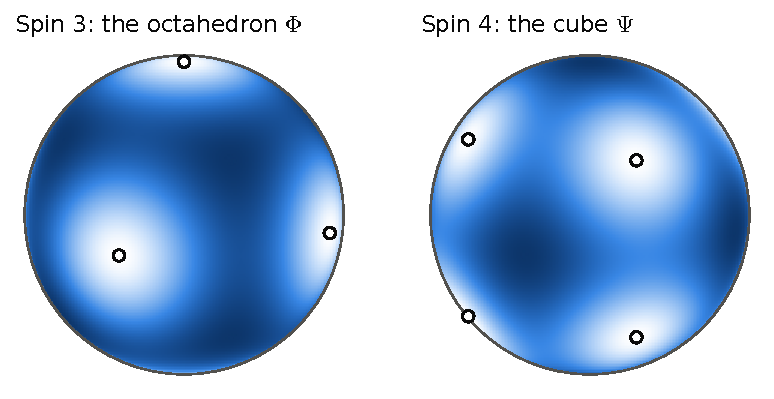
\includegraphics[width=0.74\textwidth]{spheres-constellations}
  \caption{The two smallest spin states fixed by the Hurwitz units, drawn as probability densities on the sphere (darker is larger). The circles mark the stars of the constellation, where the density vanishes: the vertices of the octahedron and of the cube.}
  \label{fig:constellations}
\end{figure}

\section{Rotating the sphere with integers}

A unit quaternion $x$ rotates space by $v\mapsto xvx^{-1}$.
The quaternions $1\pm2i$, $1\pm2j$, $1\pm2k$, of norm 5, give the rotations by the angle $\vartheta = \arccos(-\tfrac35)$ about the three axes, in both directions.

\begin{derivation}[six rotations at the Ramanujan bound]\label{d:lps}
Let $T$ send a function on the sphere to the sum of its six rotated copies.
On the harmonics of degree $l$ it is $2\big(\cos(\vartheta J_x)+\cos(\vartheta J_y)+\cos(\vartheta J_z)\big)$, with $J_x,J_y,J_z$ the angular momentum matrices of spin $l$.
On the constants $T = 6$, and on every harmonic of degree $l\ge1$ its eigenvalues satisfy
\[
  |\lambda|\le2\sqrt5
\]
(Lubotzky, Phillips and Sarnak \cite{LPS1, LPS2}; the proof rests on Deligne's bound).
The six rotations generate a free group: the $6\cdot5^{t-1}$ reduced words of length $t$ are distinct rotations.
\end{derivation}

\physical
The number $2\sqrt5$ is the norm of the same sum on the tree of the free group \cite{Kesten}.
For $l\le40$ the 1680 eigenvalues lie within $4.4475<2\sqrt5 = 4.4721$, and they follow the Kesten--McKay density $3\sqrt{20-\lambda^2}/\big(\pi(36-\lambda^2)\big)$ of the 6-regular tree \cite{McKay} to a Kolmogorov--Smirnov distance of $0.014$ (Figure~\ref{fig:rotations}).
A walk on the sphere by these rotations forgets its starting point as fast as a walk on a tree does.
A quantum bit is a point of the sphere and a gate is a rotation.
These six rotations are the V gates \cite{BGS}, and the Ramanujan bound is the reason that short circuits of such gates reach every rotation evenly \cite{ParzanchevskiSarnak}.

\begin{figure}[ht]
  \centering
  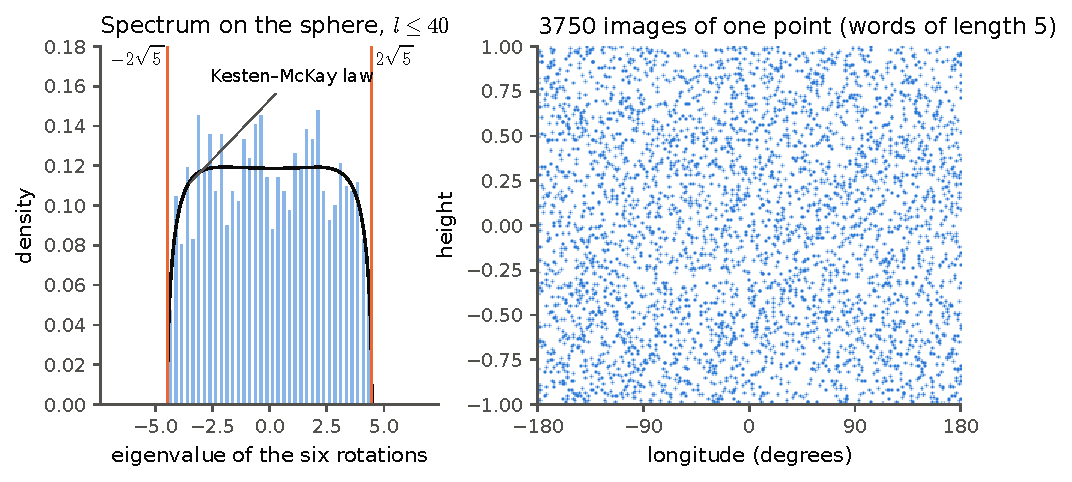
\includegraphics[width=0.94\textwidth]{spheres-rotations}
  \caption{Left: the eigenvalues of the sum of the six rotations on the harmonics of degree $1\le l\le40$, with the Kesten--McKay density and the Ramanujan bound $\pm2\sqrt5$. Right: the images of one point under the 3750 words of length 5, in coordinates where area is uniform.}
  \label{fig:rotations}
\end{figure}

\section{A working hypothesis, and questions}

Our working hypothesis is the programme of note~07 in its spherical form.
A lattice of unit impulses is analysed by radius and by angle, and modular forms carry both analyses at once: the packet of angular momentum $l$ of the shells of $\Z^d$ is a form of weight $l+d/2$, its Dirichlet series is the continuous analysis of that packet, the sizes and the squared shapes of the shells are special values of $L$-functions, and the Ramanujan bound measures how evenly the impulses are spread.

\begin{question}
The neighbours of an atom in a simple cubic crystal lie on the shells counted by $r_3(N)$, with none at the distance $\sqrt7\,a$.
Does a measurement that resolves the neighbours shell by shell, such as X-ray absorption fine structure or the crystal-field parameters of an ion, show the coefficients $a(N)$ of $\eta(z)^2\eta(2z)^7\eta(4z)^2$?
\end{question}

\begin{question}
In the four cases of Derivation~\ref{d:hurwitz} the root number of a newform of level 2 is $(-1)^j$ times the parity of a spin-$j$ state under the twist $(1+i)/\sqrt2$, a quarter turn.
Note~02 asked for a physical reading of a root number.
Is this parity one, and does the rule hold at every weight and at other levels?
\end{question}

\begin{question}
The units of $\Z$, of $\Z[\omega]$ and of the Hurwitz order are the roots of $A_1$, $A_2$ and $D_4$.
The first two are the root systems of the weak and colour forces in note~06.
Does $D_4$, with its triality, enter that programme?
\end{question}

\section*{Status of the statements}

\begin{center}
\small
\begin{tabular}{@{}p{0.64\textwidth}l@{}}
\toprule
Statement & Grade\\
\midrule
Derivations~\ref{d:packets}--\ref{d:multipoles}, \ref{d:hurwitz}(i)--(iii) and \ref{d:lps}: the cited theorems & \gradeClassical\\
Derivation~\ref{d:central}: proportionality within each class of $N$ in $\Q_2^\times$ modulo squares & \gradeClassical\\
Derivation~\ref{d:central}: one constant for the seven classes, $N\le400$; the formula for $\mu_3(N)^2$ & \gradeComputed\\
Derivation~\ref{d:hurwitz}(iii) for $\Phi,\Psi,X,\Phi^2$, and (iv) & \gradeComputed\\
Echoes: the trace identity to $10^{-13}$; $L$-value form for 151 values of $N$; silent echoes, $N\le3000$ & \gradeComputed\\
Hexadecapole identities for $d = 2,3,4$; the three eta products & \gradeComputed; theorem \gradeClassical\\
Crystal-field values $0.888\,064\,766\,485\,554$ and $1.022\,452\,1$ & \gradeComputed\\
Roundness in $d = 2,3,4$; Deligne's bound and the semicircle law for $\eta(2z)^{12}$ & \gradeComputed; theorems \gradeClassical\\
Hurwitz units as $\SL(2,\mathbb F_3)$, quotient $\Z/3$, root system $D_4$ & \gradeComputed\\
Klein's forms; the count of newforms for $l\le600$; the tetrahedral state of spin 2 & \gradeComputed; theorems \gradeClassical\\
Eigenvalues of the six rotations for $l\le40$; free group to length 6 & \gradeComputed; theorem \gradeClassical\\
The working hypothesis; Questions 1--3 & \gradeOpen\\
\bottomrule
\end{tabular}
\end{center}
\gradelegend

\begin{thebibliography}{99}
\bibitem{BanderItzykson} M.~Bander and C.~Itzykson, Group theory and the hydrogen atom (I), \emph{Rev. Mod. Phys.} 38 (1966), 330--345.
\bibitem{SatoTate} T.~Barnet-Lamb, D.~Geraghty, M.~Harris and R.~Taylor, A family of Calabi--Yau varieties and potential automorphy II, \emph{Publ. Res. Inst. Math. Sci.} 47 (2011), 29--98.
\bibitem{Bethe} H.~Bethe, Termaufspaltung in Kristallen, \emph{Ann. Phys.} 395 (1929), 133--208.
\bibitem{BGS} A.~Bocharov, Y.~Gurevich and K.~M. Svore, Efficient decomposition of single-qubit gates into $V$ basis circuits, \emph{Phys. Rev. A} 88 (2013), 012313.
\bibitem{Deligne} P.~Deligne, La conjecture de Weil. I, \emph{Publ. Math. Inst. Hautes \'Etudes Sci.} 43 (1974), 273--307.
\bibitem{DiamondShurman} F.~Diamond and J.~Shurman, \emph{A First Course in Modular Forms}, Springer, 2005.
\bibitem{Duke} W.~Duke, Hyperbolic distribution problems and half-integral weight Maass forms, \emph{Invent. Math.} 92 (1988), 73--90.
\bibitem{Eichler} M.~Eichler, The basis problem for modular forms and the traces of the Hecke operators, in \emph{Modular Functions of One Variable I}, Lecture Notes in Math. 320, Springer, 1973, 75--152.
\bibitem{Evans} L.~C. Evans, \emph{Partial Differential Equations}, 2nd ed., American Mathematical Society, 2010.
\bibitem{Ewald} P.~P. Ewald, Die Berechnung optischer und elektrostatischer Gitterpotentiale, \emph{Ann. Phys.} 369 (1921), 253--287.
\bibitem{Fock} V.~Fock, Zur Theorie des Wasserstoffatoms, \emph{Z. Phys.} 98 (1935), 145--154.
\bibitem{Grosswald} E.~Grosswald, \emph{Representations of Integers as Sums of Squares}, Springer, 1985.
\bibitem{Hecke} E.~Hecke, Eine neue Art von Zetafunktionen und ihre Beziehungen zur Verteilung der Primzahlen. Zweite Mitteilung, \emph{Math. Z.} 6 (1920), 11--51.
\bibitem{Iwaniec87} H.~Iwaniec, Fourier coefficients of modular forms of half-integral weight, \emph{Invent. Math.} 87 (1987), 385--401.
\bibitem{JacquetLanglands} H.~Jacquet and R.~P. Langlands, \emph{Automorphic Forms on $\mathrm{GL}(2)$}, Lecture Notes in Math. 114, Springer, 1970.
\bibitem{Kesten} H.~Kesten, Symmetric random walks on groups, \emph{Trans. Amer. Math. Soc.} 92 (1959), 336--354.
\bibitem{Klein} F.~Klein, \emph{Vorlesungen \"uber das Ikosaeder}, Teubner, 1884.
\bibitem{LPS1} A.~Lubotzky, R.~Phillips and P.~Sarnak, Hecke operators and distributing points on the sphere I, \emph{Comm. Pure Appl. Math.} 39 (1986), S149--S186.
\bibitem{LPS2} A.~Lubotzky, R.~Phillips and P.~Sarnak, Hecke operators and distributing points on $S^2$. II, \emph{Comm. Pure Appl. Math.} 40 (1987), 401--420.
\bibitem{Majorana} E.~Majorana, Atomi orientati in campo magnetico variabile, \emph{Nuovo Cimento} 9 (1932), 43--50.
\bibitem{McKay} B.~D. McKay, The expected eigenvalue distribution of a large regular graph, \emph{Linear Algebra Appl.} 40 (1981), 203--216.
\bibitem{ParzanchevskiSarnak} O.~Parzanchevski and P.~Sarnak, Super-golden-gates for $PU(2)$, \emph{Adv. Math.} 327 (2018), 869--901.
\bibitem{Schoeneberg} B.~Schoeneberg, Das Verhalten von mehrfachen Thetareihen bei Modulsubstitutionen, \emph{Math. Ann.} 116 (1939), 511--523.
\bibitem{Shimura} G.~Shimura, On modular forms of half integral weight, \emph{Ann. of Math.} 97 (1973), 440--481.
\bibitem{SteinWeiss} E.~M. Stein and G.~Weiss, \emph{Introduction to Fourier Analysis on Euclidean Spaces}, Princeton University Press, 1971.
\bibitem{Waldspurger} J.-L. Waldspurger, Sur les coefficients de Fourier des formes modulaires de poids demi-entier, \emph{J. Math. Pures Appl.} 60 (1981), 375--484.
\bibitem{Zagier} D.~Zagier, Modular forms and differential operators, \emph{Proc. Indian Acad. Sci. Math. Sci.} 104 (1994), 57--75.
\end{thebibliography}

\end{document}
